
Next, we propose two new variability-aware job scheduling policies, the \textit{Power Ratio Variability Prediction} and the \textit{PMC-based Variability Preciction}. These schedulers make use of the power variability prediction models introduced in Section ~\ref{sec:variability_prediction}. With these models, the schedulers predict the job's power consumption on all available sockets and schedule the job on the most efficient one. Before scheduling the job, the scheduler checks whether the system wide power budget would be respected once the job starts running. If this is not the case, the job will wait until other jobs finish and more power is available.
Additionally, we consider three job scheduling policies representative of the state-of-the-art and with increasing complexity: \textit{SLURM extended}, \textit{Power Estimation}, and \textit{Power Estimation+Variability Aware}.  The first two are variability-agnostic, while the third is variability-aware.  
Finally, we also consider an \textit{Ideal Variability Prediction}, which is based on an oracle power variability predictor that knows exactly how much power a job will consume on any processor in the system. 
We extend the SLURM's logic~\cite{slurm_02} to implement the variour power- and variability-aware job scheduling policies presented in this section. We chose SLURM as our reference because it is widely used on HPC production systems and well studied in the literature.
All job scheduling policies are described in the following:
%Next, we describe in detail all the job scheduling policies considered in this paper:

\textit{SLURM Extended}: This policy implements SLURM scheduler's logic.  We extend the default behavior to not exceed the global power budget, by considering the worst case scenario, 
which is that each job can consume the maximum power budget allowed per socket.
Additionally, we extend the scheduler to initiate backfilling for power as well~\cite{Patki:2015:PRM:2749246.2749262}.  
Traditionally, if a job requests more sockets than currently available, the scheduler will try to schedule a different job without causing delays.  
The same will happen if a job requests more power than the system can allocate.
\par
\textit{Power Estimation} (\PESched): This policy extends further \DefaultSched's behaviour by using a user provided estimation of a job's power consumption.  
For precision we obtain power profiles of previous execution of the jobs to estimate the power consumption. 
This scheduler does not consider manufacturing variability as it assumes all sockets consume the same power for a given job. 
\par
\textit{Power Estimation+Variability Aware} (\PEVASched): This policy implements elements from the state-of-the-art practices in power-aware job scheduling~\cite{Gholkar:2016:PTH:2967938.2967961,Inadomi:2015:AMI:2807591.2807638}. 
Similarly to \PESched, it estimates the power requirements of a job using a power trace from a previous execution.  
It also orders sockets and allocates first the most power efficient ones to minimize the system's net power consumption.
The socket ordering is obtained by running a simple benchmark, the cholesky kernel, on all sockets and observing their power consumption.  
A drawback of this approach is that it assumes all parallel jobs to be influenced by manufacturing variability in the very same way.
Another drawback is that a job's power estimation depends on the socket used for profiling and thus it is possible to under or over-estimate the final power.

\begin{figure}[!t]
				\centering
        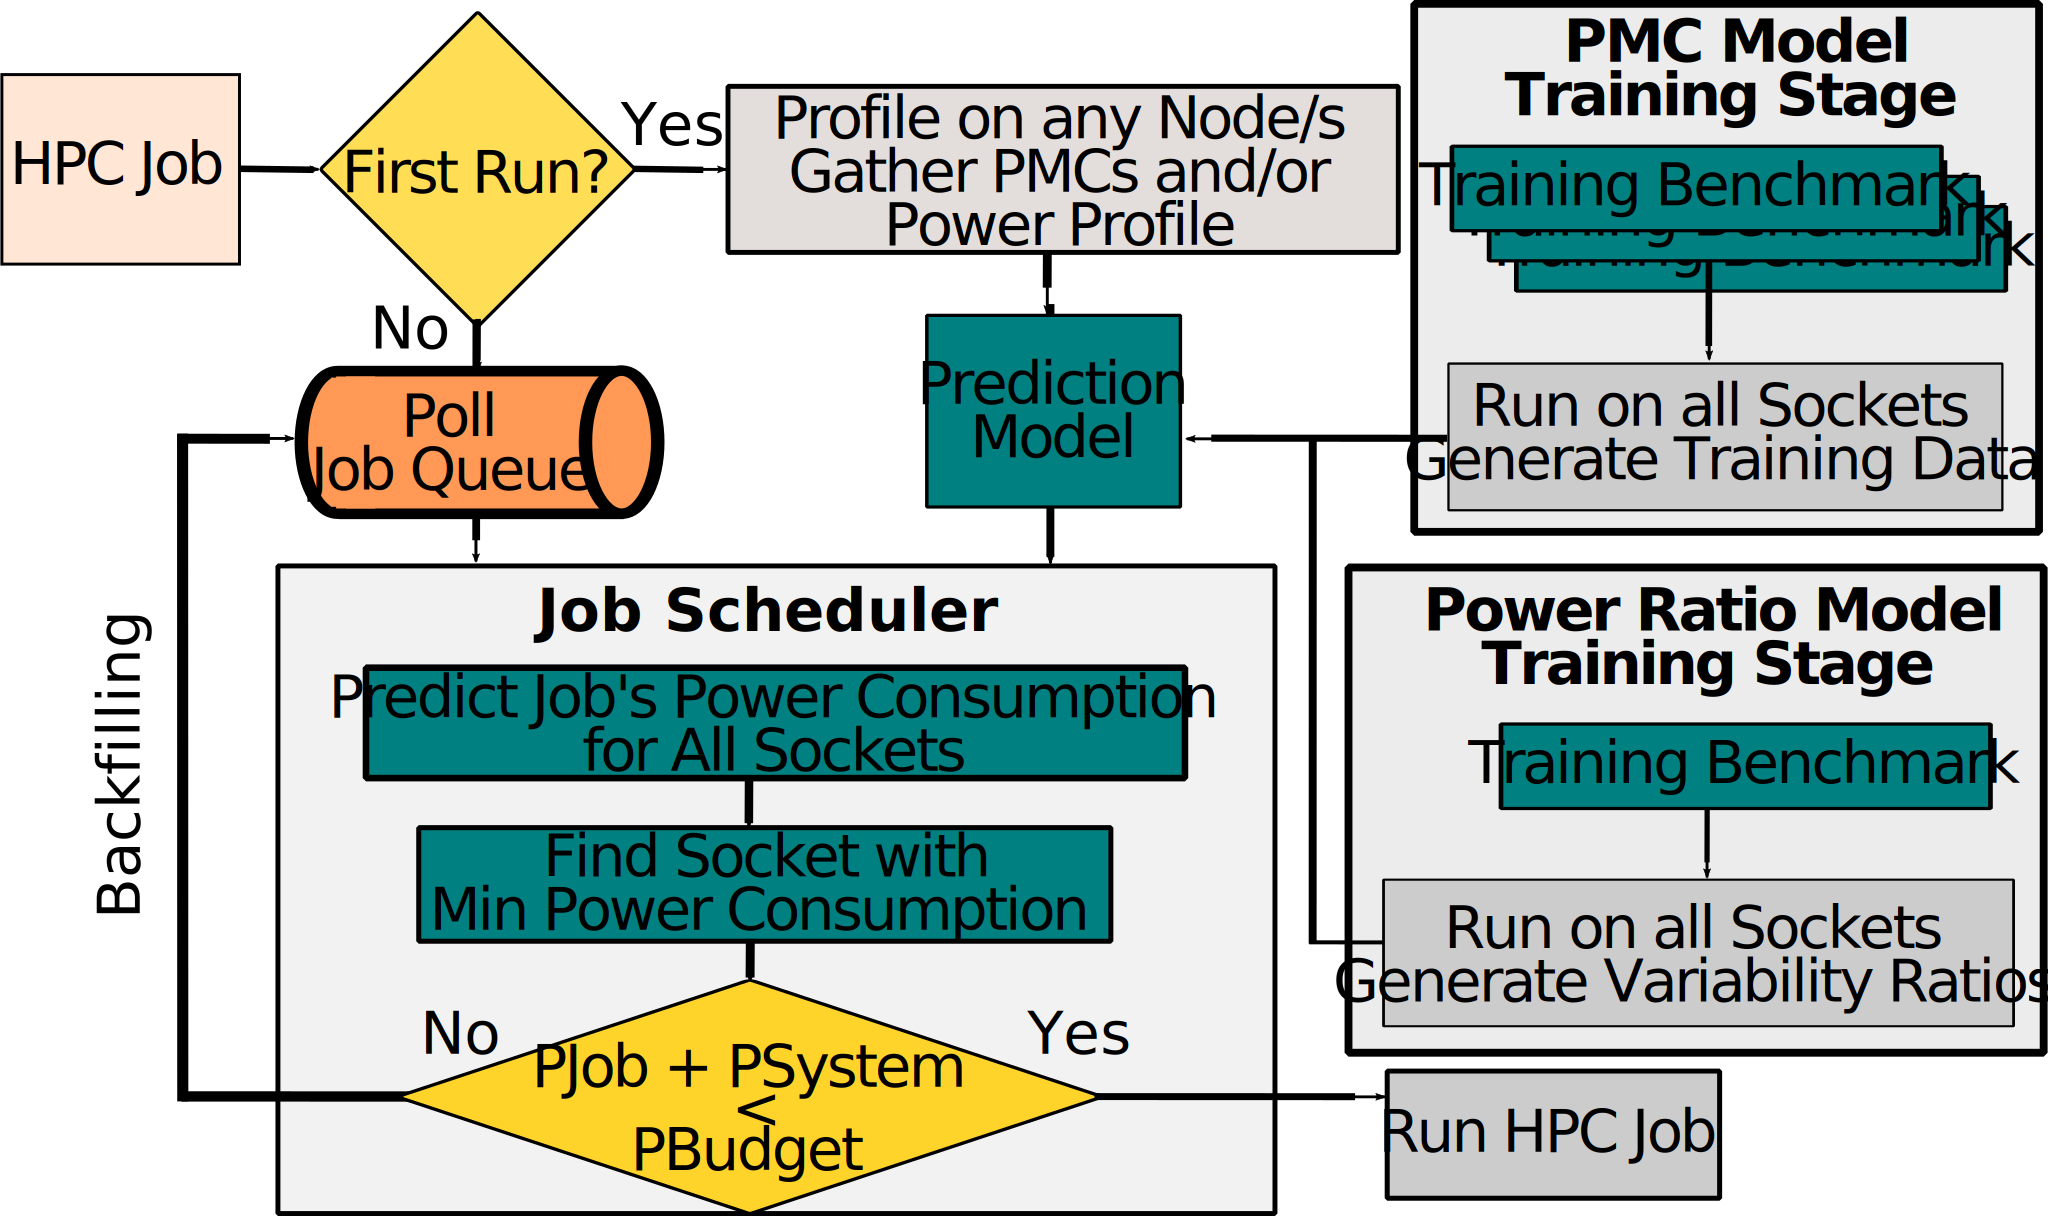
\includegraphics[width=.9\textwidth]{power_aware_job_scheduling/figures/pred_policy_recipe}
        \caption{Framework for the \PRVSSched~ and \PMCVSSched. The upper right box shows the steps for training the PMC model, while Power Ratio training stage is shown in the box below.  }
        \label{fig:pred_policy_recipe}
				\vspace{.5cm}
\end{figure}


\par
\textit{Power Ratio Variability Precition} (\PRVSSched):  This is the first new policy we propose. 
It relies on our Power Ratio Model, presented in Section~\ref{sec:naive_model}, to guide scheduling decisions.  
%To train the model, we run a single benchmark on all sockets. %Miq: not needed, already explained in 2.1
For each particular parallel job, a power trace obtained from a single run a random socket is required.
The next step is to predict the job's power consumption on all available sockets by using Equation~\ref{eq:naive_model} (presented in Section~\ref{sec:naive_model}) and choose the most efficient one.  
Moreover, if sockets are power capped, then the scheduler 
will try to find a socket where the job can run without exceeding the power limit, if possible, to avoid impacting the job's performance.
The predictions are also used to determine the net power consumption of the whole system and maintaining it below the global power budget. 
If the predicted power for a new job makes the system budget to go over its limit,
then the job waits until resources are released.  
The backfilling scheme is the same as with the previous policies. 
This policy's framework is shown in Figure~\ref{fig:pred_policy_recipe}.  
Note that two training processes are shown in the figure, for the different power 
prediction models proposed in this work.  The lower box shows corresponds to the \PRVSSched~ policy.

\begin{figure*}[ht!]
	\centering
	\begin{subfigure}[b]{.9\textwidth}
		\includegraphics[width=\textwidth]{power_aware_job_scheduling/figures/model_power_pred_error}
		\caption{Power prediction error for all models}
		\label{fig:model_power_pred_error}
	\end{subfigure}%
	
	\begin{subfigure}[b]{.9\textwidth}
		\includegraphics[width=\textwidth]{power_aware_job_scheduling/figures/model_peak_pred_error}
		\caption{Peak power prediction error for all models}
		\label{fig:model_peak_pred_error}
	\end{subfigure}%
	\caption{Comparison of average power prediction error for all models (left figure) over all sockets.  
					Right figure shows the average prediction error only for the peak power consumption each application can reach.  
					The error bars show the standard error deviation across all sockets for the corresponding application.}
					\vspace{.5cm}
\end{figure*}

\par
\textit{PMC-based Variability Prediction} (\PMCVSSched): Our second proposed policy is similar to the PRVS policy, but it uses our \textit{Optimized PMC Model}, presented in Section~\ref{sec:pmcs_model}, to obtain power consumption predictions\footnote{The \textit{Generic PMC} model is not used due to its poor prediction capabilities, which are shown in Section~\ref{sec:model_validation}.}.  
This policy requires running the training benchmark set from Table~\ref{tab:training_set} on all sockets in order to train the model.  
A single power profile of a given job (or one for each socket a process was run on, in the case of multi-node jobs) is also required in order to compute the activity ratios, which can be performed on any set of sockets in the system. Single-node jobs only require a single socket of the whole system, however multi-node jobs needs to be run on at least $N$ sockets, where $N$ is the number of socket required by the job.
 With this profile, power predictions per available socket are obtained, and scheduling decisions are made in the
same manner as with the \PRVSSched~ approach. 
The framework for this policy is described in Figure~\ref{fig:pred_policy_recipe}. 
The box on the upper right corner corresponds to the training process of the \textit{PMC-based Prediction Models}, used by \PMCVSSched.
\par
\textit{Ideal Variability Preciction} (\IVSSched): Identical to \PRVSSched~ and \PMCVSSched, but using an oracle power predictor to drive job scheduling decisions. 
This policy is aimed at showing the impact of using a 100\% accurate model to guide scheduling decisions. Thus, \IVSSched~ is used for comparison purposes to show the maximum benefits that can be achieved by power- and variability-aware job scheduling policies.

